\documentclass[12pt,a4paper]{article}

% Language setting
\usepackage[british]{babel}

% Set page size and margins
\usepackage[a4paper,top=2cm,bottom=2cm,left=2.5cm,right=2.5cm,marginparwidth=1.75cm]{geometry}

%----------- APA style references & citations (starting) ---
% Useful packages
%\usepackage[natbibapa]{apacite} % APA-style citations.

\usepackage[style=apa, backend=biber]{biblatex} % APA 7th edition style citations using biblatex
\addbibresource{references.bib} % Your .bib file

% Formatting DOI in APA-7 style
%\renewcommand{\doiprefix}{https://doi.org/}

% Add additional APA 7th edition requirements
\DeclareLanguageMapping{british}{british-apa} % Set language mapping
\DeclareFieldFormat[article]{volume}{\apanum{#1}} % Format volume number

% Modify 'and' to '&' in the bibliography
\renewcommand*{\finalnamedelim}{%
  \ifnumgreater{\value{liststop}}{2}{\finalandcomma}{}%
  \addspace\&\space}
  
%----------- APA style references & citations (ending) ---


\usepackage{amsmath}
\usepackage{graphicx}
\usepackage[colorlinks=true, allcolors=blue]{hyperref}
\usepackage{hyperref}
\usepackage{orcidlink}
\usepackage[title]{appendix}
\usepackage{mathrsfs}
\usepackage{amsfonts}
\usepackage{booktabs} % For \toprule, \midrule, \botrule
\usepackage{caption}  % For \caption
\usepackage{threeparttable} % For table footnotes
\usepackage{algorithm}
\usepackage{algorithmicx}
\usepackage{algpseudocode}
\usepackage{listings}
\usepackage{enumitem}
\usepackage{chngcntr}
\usepackage{booktabs}
\usepackage{lipsum}
\usepackage{subcaption}
\usepackage{authblk}
\usepackage[T1]{fontenc}    % Font encoding
\usepackage{csquotes}       % Include csquotes
\usepackage{diagbox}
\usepackage{listings}
\usepackage{xcolor}

%%% Code containers:
\definecolor{codegreen}{rgb}{0,0.6,0}
\definecolor{codegray}{rgb}{0.5,0.5,0.5}
\definecolor{codepurple}{rgb}{0.58,0,0.82}
\definecolor{backcolour}{rgb}{0.95,0.95,0.92}

\lstdefinestyle{mystyle}{
    backgroundcolor=\color{backcolour},   
    commentstyle=\color{codegreen},
    keywordstyle=\color{magenta},
    numberstyle=\tiny\color{codegray},
    stringstyle=\color{codepurple},
    basicstyle=\ttfamily\footnotesize,
    breakatwhitespace=false,         
    breaklines=true,                 
    captionpos=b,                    
    keepspaces=true,                 
    numbers=left,                    
    numbersep=5pt,                  
    showspaces=false,                
    showstringspaces=false,
    showtabs=false,                  
    tabsize=2
}

\lstset{style=mystyle}


%%% Box quotes:
% for adjustwidth environment
\usepackage[strict]{changepage}

% for formal definitions
\usepackage{framed}

% environment derived from framed.sty: see leftbar environment definition
\definecolor{formalshade}{rgb}{0.95,0.95,1}

\newenvironment{formal}{%
  \def\FrameCommand{%
    \hspace{1pt}%
    {\color{codegreen}\vrule width 2pt}%
    {\color{formalshade}\vrule width 4pt}%
    \colorbox{formalshade}%
  }%
  \MakeFramed{\advance\hsize-\width\FrameRestore}%
  \noindent\hspace{-4.55pt}% disable indenting first paragraph
  \begin{adjustwidth}{}{7pt}%
  \vspace{2pt}\vspace{2pt}%
}
{%
  \vspace{2pt}\end{adjustwidth}\endMakeFramed%
}


% Customize line spacing
\usepackage{setspace}
\onehalfspacing % 1.5 line spacing

% Redefine section and subsection numbering format
\usepackage{titlesec}
\titleformat{\section} % Redefine section numbering format
  {\normalfont\Large\bfseries}{\thesection.}{1em}{}
  
% Customize line numbering format to right-align line numbers
\usepackage{lineno} % Add the lineno package
\renewcommand\linenumberfont{\normalfont\scriptsize\sffamily\color{blue}}
\rightlinenumbers % Right-align line numbers

\linenumbers % Enable line numbering

% Define a new command for the fourth-level title.
\newcommand{\subsubsubsection}[1]{%
  \vspace{\baselineskip}% Add some space
  \noindent\textbf{#1\\}\quad% Adjust formatting as needed
}
% Change the position of the table caption above the table
\usepackage{float}   % for customizing caption position
\usepackage{caption} % for customizing caption format
\captionsetup[table]{position=top} % caption position for tables

% Define the unnumbered list
\makeatletter
\newenvironment{unlist}{%
  \begin{list}{}{%
    \setlength{\labelwidth}{0pt}%
    \setlength{\labelsep}{0pt}%
    \setlength{\leftmargin}{2em}%
    \setlength{\itemindent}{-2em}%
    \setlength{\topsep}{\medskipamount}%
    \setlength{\itemsep}{3pt}%
  }%
}{%
  \end{list}%
}
\makeatother

% Suppress the warning about \@parboxrestore
\pdfsuppresswarningpagegroup=1


%-------------------------------------------
% Paper Head
%-------------------------------------------
\title{ChatGPT Performance Analysis on Annotation Tasks}

\author{Leonardo Matone}

\date{}  % Remove date

\begin{document}
\maketitle

\begin{abstract} \noindent Many Natural Language Processing (NLP) applications require labeled data which is both time consuming and expensive. Projects of large scope usually require many manual coders, and niche areas of study require these coders to have a degree of training or knowledge of the field. The advance of Large Language Models (LLMs) in the past decade have led to huge improvements in language processing and comprehension. Chatbots like ChatGPT are capable of outperforming annotators on specific datasets, and their zero-shot accuracy provide compelling evidence that LLMs could be the future of text annotation. This study will be focused on three things: (1) how well does ChatGPT compare to human coders on a multi-class problem, (2) how does it compare against other NLP approaches and (3) with slight prompt engineering and a few pre-training steps, does the ChatGPT approach offer efficiency benefits over the industry standards? 
%\lipsum[1]
\end{abstract}

\textbf{Keywords}: ChatGPT, Text Annotation  

%-------------------------------------------
% Paper Body
%-------------------------------------------


%--- Section ---%
\section{Problem Overview}

\noindent NLP tasks often require large amounts of labeled data. Modern classification approaches are heavily resource intensive and require labels to compute their gradients, and unsupervised models require labels to quantify their accuracy. ChatGPT has been demonstrated to outperform human coders on certain tasks (Gilardi et al.), but has not been compared against NLP approaches to the same task. This report is concerned with the following: 

\begin{enumerate}
  \item How well do ChatGPT's zero-shot and fine-tuned models hold up against an NLP model trained on the same task, with the same labeled data?
  \item What forms should prompt-engineering on multi-class classification problems take?
  \item How much fine-tuning can be generalized to an unseen domain?
\end{enumerate}

\noindent LLMs have demonstated their ability to perform very well across domains. this project aims to explore the power of ChatGPT in annotation tasks by comparing their representative power against other NLP approaches. It also aims to evaluate the best methods of prompt-engineering and fine-tuning with a lens for unseen domains. \\



%--- Section ---%
\section{Data}\label{sec2}

\noindent The data for this project is a collection of reviews from New Orleans schools. The data was collected and annotated by the Tulane Economics Department, and consists of 500 student-annotated reviews, categorized into level 1 and level 2 categories, with level 2 denoting higher specificity and complexity. There are manual annotations from student-coders for the level 1 categories, which include: school-level features, physical environment, instruction \& learning, school staff, overall quality, school culture, and resources. Manual coders were instructed to label each review with all applicable level 1 categories. The data also includes level 1 classifications from the Tulane Economics Department's NLP model for these 500 reviews. A version of this dataset exists in this report's \href{https://github.com/tulane-cmps6730/project-polititweet}{GitHub repository}.\\

\noindent There are two datasets which are merged by index for the purposes of this project. The first contains the annotations from the human coders and the NLP model, and the second contains the actual reviews and other relevant information per review. The dataset available in the project's GitHub is the merged dataset consisting of both sources. 



%--- Section ---%
\section{Methods}\label{sec3}

\noindent To perform classification on the review dataset, we designed an interface layer to interact with \href{https://platform.openai.com/docs/overview}{OpenAI's API}. Because ChatGPT is inherently creative and chooses its output stochastically based on the input, the format of the output must be standardized. In our testing, we did extensive prompt-engineering with the goal of encouraging accuracy but also standardizing output. Our initial interface layer would work sporadically, the stochastic nature of the output (both in terms of predictions and formatting) made this unreliable. Instead of penalizing incorrect response formats (as with a large enough token count on the review, ChatGPT seems to focus on directions less), we specify a limitation on stochastic responses in each API call using a \'temperature\' and \'top\_p\' setting of 0.1 and 0.2, respectively. Temperature denotes the creativity and randomness of the response. ChatGPT has been trained to handle a variety of tasks from code to text generation, and both require different character-level stochastic settings. By specifying the temperature as 0.1, we encourage the model be less random and more reliable, as is expected when ChatGPT produces code. Similarly, top\_p represents the top token probability mass, the lower we set this, the less variance in our response. \\

\noindent Our interface layer allows for wiggle-room in how ChatGPT receives our unlabeled text and what prompt and categories it is given. The default prompt is: 

\begin{lstlisting}
"Which of these topics: {topics} are discussed in this review: {text}. 
For all topics, respond in the format: "topic": 0 or 1."
\end{lstlisting} \\

\noindent Our initial comparisons will use no prompt engineering or fine-tuning in order to estimate ChatGPT's zero-shot capabilities in full. We will compare against the Tulane Economics Department's NLP model and human coders, and then begin optimizing this LLM approach.


%--- Section ---%
\section{Preliminary Experiments \& Results}\label{sec4}

\noindent We have completed a series of small experiments concerned with establishing a functional input layer and several rudimentary analyses of the results against existing NLP approaches and human-coded annotations. Each is labeled 1-4 in this project's GitHub repository, under \href{https://github.com/tulane-cmps6730/project-polititweet/tree/main/notebooks}{notebooks}.


\subsection{Preliminary Evaluation}
\noindent As a first test, we used OpenAI's API to interact with ChatGPT and feed it a single review. We use the level 1 categories defined by the Tulane Econommics Department which consist of \textit{school-level features}, \textit{physical environment}, \textit{instruction \& learning}, \textit{school staff}, \textit{overall quality}, \textit{school culture}, and \textit{resources}. Below is the sample we passed to ChatGPT 3.5 and ChatGPT 4.0.

\begin{formal}
(PLEASE DONOT SEND YOUR KIDS HERE) LOTS OF BULLYING AND FIGHTS I went here when I was a kid and it was bad and now it is worst as it has ever been I well adment the teachers are ok I loved Mrs.Long and Mrs.Right but there were lots of fights and lots of people in my class was below grade level and had 50's,40's,30's,and even F's SO I would just like everyone to know about this school.Thanks\\
\end{formal}

\noindent This review is a good example of some of the NLP challenges which make learning from such data difficult. The formatting is inconsistent, at times the user is ambiguous, and some of the categories themselves are questionably general. From Table 1 below, it is evident that GPT is not going to always match our source of truth, the human annotators. Arguably, the results of GPT's labeling are comparable, which is what the existing literature would have us believe. In this case, Both GPT models annotated "Student discipline" as 1, which is implicit to a human reader from the review, but for whatever reason the human annotators did not flag it. Either way, the performance of both GPTs seems to leave something to be desired.\\

\begin{table}[htb]
    \caption{ChatGPT 3.5/4.0 Predictions for 1 Review\label{tab1}}
    
    \begin{tabular*}{\columnwidth}{@{\extracolsep\fill}llll@{\extracolsep\fill}}
        \toprule
        Category & hum & 3.5 & 4.0 \\
        \midrule
        Student discipline & 0 & 1 & 1 \\
        Teacher quality & 0 & 1 & 1 \\
        School culture & 0 & 0 & 1 \\
        Building quality & 0 & 0 & 0 \\
        School staff & 1 & 0 & 1 \\
        Instruction & 1 & 0 & 0 \\
        School safety & 1 & 0 & 1 \\
        \bottomrule
    \end{tabular*}
    \begin{tablenotes}
        \item *results of preliminary test
    \end{tablenotes}

\end{table}


\subsection{Interface Layer}

\noindent To make a prediction over all 500 of our labeled reviews, we designed an interface layer to query OpenAI's API and retrieve a prediction for each record. After combining the NLP/human coded dataset with the full dataset containing all review documents, we ran a test on a subset of 20 records. Each test has a real-world cost in OpenAI's payment heirarchy, so testing was limited in this stage. The cost scales with token counts, so this stage includes no prompt-engineering. On the level 1 categories, we compute the Jaccard similarities between the manually annotated reviews and ChatGPT 3.5 and ChatGPT 4.0's annotations, which you can see in Figure 1 (final report will have larger font and alpha to better see comparison):

\begin{figure}[H]
    \centering
    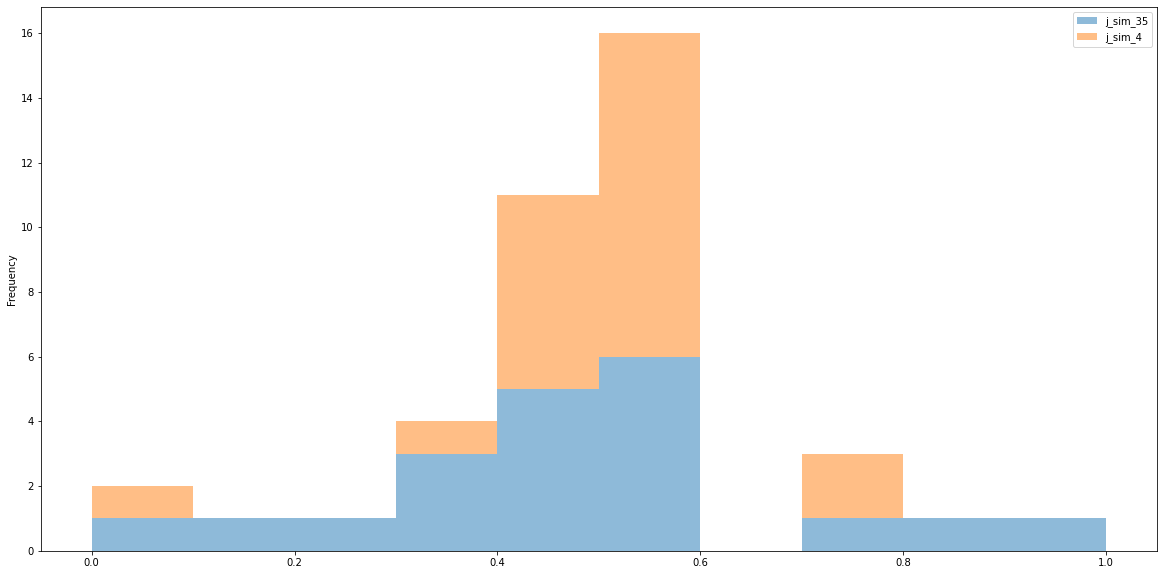
\includegraphics[width=1.0\linewidth]{jaccard_similarity_20.png}
    \caption{Jaccard Scores for 3.5 and 4.0}
    \label{fig1:Jaccard Scores for 3.5 and 4.0}
\end{figure}

\noindent An interesting discovery in this experiment is the impact of tokens on the output of GPT 3.5 \& 4.0. Both output different results based on the length and content of the review as they should, but often will make different guesses with subsequent calls for the same review. This is due to the stochastic nature of the output, which, even with our passed temperature and top\_p parameters, cannot be stifled permanently without fine-tuning or inflating our token counts to specify formatting in-depth. The final report will take steps to experiment with both of these alternatives. 


\subsection{Full Test}

\noindent With our preliminary tests and interface layer complete, we ran ChatGPT 3.5 ad ChatGPT 4.0 on the full dataset of 500 reviews. This is a time-intensive and high-cost endeavor (taking ~30 minutes and costing ~\$5.00 in total), which we will aim to replicate at most 2 more times to compare prompt-engineering approaches. This first full test yielded unexpectedly low results, which are summarized in Table 2. The accuracy and precision of both LLMs is much lower than the NLP model, and while this is zero-shot learning, the existing literature would lead us to expect better results. Recall is slightly higher for both LLMs, as shown in Table 2. This is likely due to the increased variance in false negatives and false positives compared to the NLP model, shown in Figure 2. It is evident that the NLP model has been tuned to avoid false positives, and both GPT models try to get every category that could be in the review, perhaps defaultly prioritizing recall. \\

\begin{table}[htb]
    \caption{Model Performance Comparison\label{tab2}}
    \centering
    \scalebox{0.92}{% Scale the table to 75% of the original size
        \begin{tabular}{lccccc}
        \toprule
        Name & Jaccard Score & Recall Score & Precision Score & F1 Score & Accuracy Score \\
        \midrule
        coded & 0.995976 & 0.995976 & 0.995976 & 0.995976 & 1.000000 \\
        nlp\_df & 0.583252 & 0.623259 & 0.877005 & 0.704345 & 0.735844 \\
        predictions\_35\_df & 0.479884 & 0.653679 & 0.672789 & 0.607320 & 0.603334 \\
        predictions\_40\_df & 0.511953 & 0.692795 & 0.683396 & 0.647616 & 0.620868 \\
        \bottomrule
        \end{tabular}
    } % End scalebox
    \label{tab:model_performance}
\end{table}

\begin{figure}[H]
    \centering
    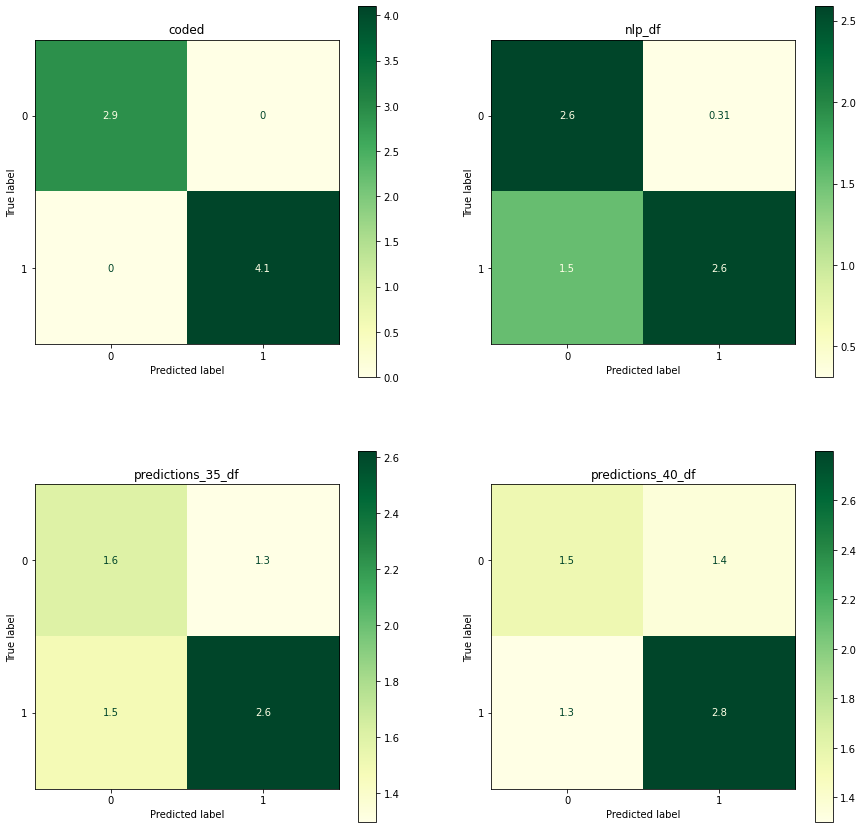
\includegraphics[width=1.0\linewidth]{avg_confusion_matrix_full.png}
    \caption{Averaged Confusion Matrices}
    \label{fig:enter-label}
\end{figure}


\subsection{Category Analysis}

\noindent Figure 2 illustrates the averaged confusion matrices across all 500 predictions. We studied each category's confusion matrices independently to evaluate where OpenAI's strengths and weaknesses lie across 3.5 and 4.0. We found that GPT's interpretation of labels in its prompt fall into three categories: unclear comprehension, clear comprehension, and somewhat-clear comprehension. The deciding factors for each of these categories are the ambiguity and/or expressiveness of the label's terms. \\

\begin{figure}[H]
    \centering
    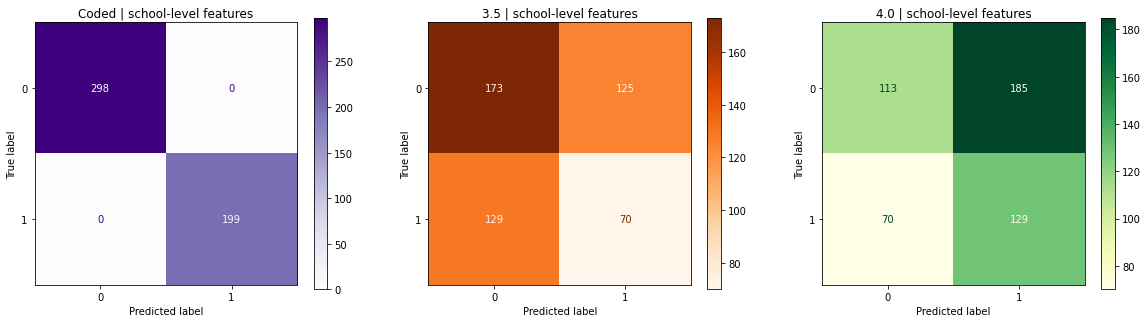
\includegraphics[width=1\linewidth]{school_level_features_confusion.png}
    \caption{Unclear Comprehension (School-Level Features)}
    \label{fig:enter-label}
\end{figure}

\noindent Unlike the NLP model, ChatGPT has virtually the same amount of information the human coders received. It understands the name of the label, and attempts to understand which reviews contain the label solely based on the language embedding it accumulated from training. Thus, more ambiguous labels like "school-level features" or "resources" suffer in accuracy and experience confusion, even between 3.5 and 4.0. This is evident in Figure 3, where 3.5 and 4.0 have wildly different understandings of what "school-level features" means, exhibiting different trends in how they label and varying wildly across false positives and false negatives.\\

\begin{figure}[H]
    \centering
    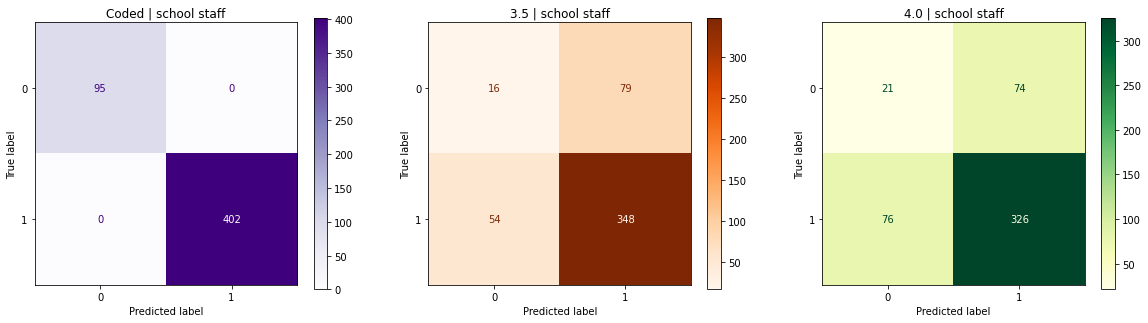
\includegraphics[width=1\linewidth]{school_staff_confusion_full.png}
    \caption{Clear Comprehension (School Staff)}
    \label{fig:enter-label}
\end{figure}

\noindent As illustrated in Figure 4, "School Staff" is an example of a more interpretable label, with far less variance across false negatives and false positives. Figure 5 illustrates somewhat-clear comprehension. While both models tend to label positively like the coders, there is greater variance in false positives and negatives.\\

\begin{figure}[H]
    \centering
    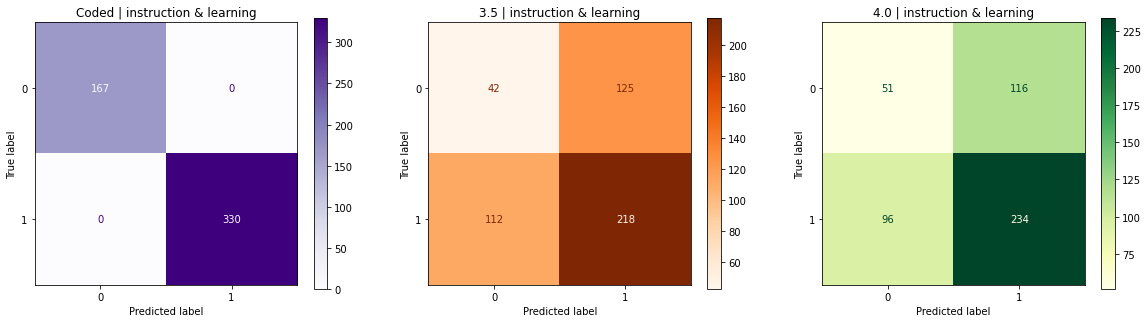
\includegraphics[width=1\linewidth]{instruction_and_learning_confusion_full.png}
    \caption{Somewhat Clear Comprehension (Instruction \& Learning}
    \label{fig:enter-label}
\end{figure}


%--- Section ---%
\section{Related Work}\label{sec5}

\noindent Considering the relative youth of ChatGPT, there have been a considerable number of papers written studying the use of ChatGPT as an annotator. The primary example of which has already been cited. \textit{Gilardi et al}. demonstrate that ChatGPT can outperform MTurk annotators. Running a similar experiment, they compared the results of ChatGPT's annotation against the human annotations from MTurk, using a gold-standard annotation from research assistants as their source of truth. Their experiments were conducted on a range of tasks, ranging from binary to multi-class classification. Their results indicate that ChatGPT is well suited to annotation tasks, but do not compare the approach of ChatGPT against existing NLP approaches. Additionally, they do not fine-tune or experiment with prompt-engineering. They utilize ChatGPT's zero-shot learning alone. \\

\noindent \textit{Dai et al.} introduce a method to use ChatGPT for generating new text data, aimed at augmenting existing datasets to improve model training in text classification. It explores various data augmentation techniques at character, word, and sentence levels, emphasizing the importance of generating diverse and semantically consistent samples to enhance the robustness and performance of NLP models. While this is related to this project as both intend to augment and upgrade the availability of text data for learning, this is a different area altogether.\\ 

\noindent \textit{Wang et al.} illustrate ChatGPT 3.5 as a cost-effective solution for data labeling, highlighting its potential to significantly reduce expenses compared to traditional human labeling while maintaining a high level of data quality. It explores the process of using ChatGPT 3.5 for labeling and the implications for cost, efficiency, and model performance, suggesting that leveraging ChatGPT 3.5 could work well for data annotation tasks. This article is a precursor to \textit{Gilardi et al}, and while it is part of the relevant literature it is unrelated to this project's goals for the same reason.\\ 

\noindent \textit{Kuzman et al.} focus on the domain of automatic genre identification. The study investigates ChatGPT's capabilities against traditional NLP models. By annotating text data with genre labels and comparing the performance of ChatGPT with a multilingual transformer-based model, the paper explores the potential of large language models to streamline or even replace manual annotation processes in specific contexts, signifying a shift towards more efficient and automated methods of data labeling. This is very close to what we aim to accomplish with this project, but like \textit{Gilardi et al}, they do not fine-tune or perform any prompt-engineering, instead studying the zero-shot learning capabilities of ChatGPT.\\

\noindent \textit{Huang et al.} examine ChatGPT's effectiveness compared to human annotators in identifying implicit hate speech, a nuanced and complex task. Their findings delve into ChatGPT's potential advantages and its limitations, suggesting that while ChatGPT shows promise in automating the detection of such content, it may not fully grasp the subtleties that human annotators can discern. This paper illustrates the domain limitations on ChatGPT, and the fact that it struggles in certain environments due to its inherent bias. 

\section{Timeline}

\noindent There are two more planned steps to this project. First, we will perform prompt-engineering and fine-tuning steps to examine how well ChatGPT holds up to NLP approaches. We will perform these steps with a lens for generalization on this task across domains, withholding domain-specific information. This is with the intention of our second step, which is the application of this ChatGPT to an unseen labeled domain to assess the generalization of a fine-tuned ChatGPT model.

\section{References}

\noindent Gilardi, F., Alizadeh, M., \& Kubli, M. (2023). ChatGPT outperforms crowd workers for  \\
\indent text-annotation tasks. Proceedings of the National Academy of Sciences, 120(30). ht- \\
\indent tps://arxiv.org/abs/2303.15056 \\ 

\noindent Haixing Dai, Zhengliang Liu, Wenxiong Liao, Xiaoke Huang, Yihan Cao, Zihao Wu, Lin \\
\indent Zhao, Shaochen Xu, Wei Liu, Ninghao Liu, Sheng Li, Dajiang Zhu, Hongmin Cai, \\
\indent Lichao Sun, Quanzheng Li, Dinggang Shen, Tianming Liu, \& Xiang Li. (2023). Aug- \\
\indent GPT: Leveraging ChatGPT for Text Data Augmentation. https://arxiv.org/abs/2302.13007 \\

\noindent Shuohang Wang, Yang Liu, Yichong Xu, Chenguang Zhu, \& Michael Zeng. (2021). Want \\
\indent To Reduce Labeling Cost? GPT-3 Can Help. https://arxiv.org/abs/2108.13487 \\

\noindent Taja Kuzman, Igor Mozetič, \& Nikola Ljubešić. (2023). ChatGPT: Beginning of an End \\
\indent of Manual Linguistic Data Annotation? Use Case of Automatic Genre Identification. https://arxiv.org/abs/2303.03953 \\ 

\noindent Huang, F., Kwak, H., \& An, J. (2023). Is ChatGPT better than Human Annotators? Po- \\
\indent tential and Limitations of ChatGPT in Explaining Implicit Hate Speech. In Compani-\\
\indent on Proceedings of the ACM Web Conference 2023. ACM. \\





\end{document}